\documentclass{PiMart}    % 2017/12/5: created the file by Dingquan Li, email: dingquanli@pku.edu.cn
%----user-defined----
%----user-defined end----
%%%%%%%%%%%%%%%%%%%%%%%%%%%%%%%%%%%%%%%%%%%%%%%%%%%%%%%%%%%%%%%%%%%%%%%%%%%%%%%%%%%%%%%%
%%------------------ Information offered by the editorial office ---------------------%%
%%%%%%%%%%%%%%%%%%%%%%%%%%%%%%%%%%%%%%%%%%%%%%%%%%%%%%%%%%%%%%%%%%%%%%%%%%%%%%%%%%%%%%%%
\newcommand{\pubvol}{46} % Vol.
\newcommand{\pubno}{4} % No.
\newcommand{\pubyear}{2017} % Year
\newcommand{\pubmonth}{7} % Month
\newcommand{\spage}{583} % Start page
\newcommand{\epage}{586} % End page
\newcommand{\submitinfo}{Received~June 5, 2015; revised July 17, 2016} % Received, Revised
%%
%%%%%%%%%%%%%%%%%%%%%%%%%%%%%%%%%%%%%%%%%%%%%%%%%%%%%%%%%%%%%%%%%%%%%%%%%%%%%%%%%%%%%
%%-------------------- Information provided by the authors ------------------------%%
%%%%%%%%%%%%%%%%%%%%%%%%%%%%%%%%%%%%%%%%%%%%%%%%%%%%%%%%%%%%%%%%%%%%%%%%%%%%%%%%%%%%%
%%
\newcommand{\entitle}{Sample Article of PiM} % Title
\newcommand{\shorttitle}{Sample Article of PiM}  % Short Title for Header
\newcommand{\enauthor}{LI Dingquan$^{1,2}$, NIU Kaifu$^{1,2}$ and YANG Fengxia$^{1,2,\star}$} % Author
\newcommand{\shortauthor}{LI D., NIU K. and YANG F.} % Short Author for Header
\newcommand{\eninstitution}{$^1$School of Mathematical Sciences, Peking University, Beijing, 100871, P. R. China\\$^2$LMAM} % Institution
\newcommand{\enabstract}{Bla, Bla, Bla, Bla, Bla, Bla, Bla, Bla, Bla, Bla, Bla, Bla, Bla, Bla, Bla, Bla, Bla, Bla, Bla, Bla, Bla, Bla, Bla, Bla, Bla, Bla, Bla, Bla, Bla, Bla, Bla, Bla, Bla.} % Abstract
\newcommand{\enkeywords}{BlaBlaBla, BlaBlaBla, BlaBlaBla} % Keywords
%%
\newcommand{\MR}{} % MR(2010) Subject Classification
\newcommand{\fundinfo}{The work is supported by } % Funding
\newcommand{\authorinfo}{yangfx@math.pku.edu.cn ($^\star$Corresponding Author)} % E-mail
\newcommand{\authorthanks}{The authors thank the referees for their valuable comments and suggestions.} % Acknowledgements
%%%%%%%%%%%%%%%%%%%%%%%%%%%%%%%%%%%%%%%%%%%%%%%%%%%%%%%%%%%%%%%%%%%%%%%%%%%%%%%%%%%%%%%%%%%%%%%%%%%%%%%%%
%%%%%%%%%%%%%%%%%%%%%%%%%%%%%%%%%%%%%%%%%%%%%%%%%%%%%%%%%%%%%%%%%%%%%%%%%%%%%%%%%%%%%%%%%%%%%%%%%%%%%%%%%
\begin{document}
\maketitle
%%%%%%%%%%%%%%%%%%%%%%%%%%%%%%%%%%% Mainbody
\section{Introduction}\label{sec:Intro}
\begin{itemize}
\item Section~\ref{sec:theorem}: Theorem
\item Section~\ref{sec:citeref}: Cite, Ref
\end{itemize}
Bla, Bla, Bla, Bla, Bla, Bla, Bla, Bla, Bla, Bla, Bla, Bla, Bla, Bla, Bla, Bla, Bla, Bla, Bla, Bla, Bla, Bla, Bla, Bla, Bla, Bla, Bla, Bla, Bla, Bla, Bla, Bla, Bla.
\subsection{Subsection}
\subsubsection{Subsubsection}
Bla, Bla, Bla, Bla, Bla, Bla, Bla, Bla, Bla, Bla, Bla, Bla, Bla, Bla, Bla, Bla, Bla, Bla, Bla, Bla, Bla, Bl.
\section{Theorem Env.} \label{sec:theorem}
\begin{theorem}\label{thm:a}
Theorem
\end{theorem}
\begin{theorem}[\cite{[1]}]
Theorem
\end{theorem}
\begin{lemma}[{\cite[Theorem~2]{[5]}}]
Lemma
\end{lemma}
\begin{corollary}\label{cor:a}
Corollary
\end{corollary}
\begin{definition}[XXX]\label{def:a}
Definition
\end{definition}

\begin{remark}[\cite{[1]}]
Remark
\end{remark}
\begin{problem}
Problem
\end{problem}
\begin{example}
Example
\end{example}

Other env.: proposition, conjecture, algorithm, property; question, hypothesis, case

\begin{proof}
Proof
\end{proof}

\section{cite, label/tag/ref/eqref}\label{sec:citeref}

Reference Citation~\cite{[1],[2],[3],[4]}

Equation: Eq.~(\ref{eq:1}) or Eq.~\eqref{eq:1}

Table~\ref{tab:1}, Figure~\ref{fig:fig4}, Figure~\ref{fig:float2-1}, Figure~\ref{fig:mini:subfig:a}

\begin{equation}\label{eq:1}
\left\{\begin{aligned}
&x(t)=S_\alpha(t)[x_0-g(x)]+\int_0^tS_\alpha(t-s)[f(s,x(s))+Bu(s)]\mathrm{d}s,\quad 0\leq t\leq b,\\
&u(t)=B^*S_\alpha^*(b-t)R(\lambda,\Lambda_b)p(x(\,\cdot\,)),\\
&p(x(\,\cdot\,))=x_b-S_\alpha(b)[x_0-g(x)]-\int_0^bS_\alpha(b-s)f(s,x(s))\mathrm{d}s.
\end{aligned}
\right.
\end{equation}

\begin{table}[!htb]\label{tab:1}
\centering
\caption{XXX}
\vspace{2mm}
\begin{tabular}{ccclc}
\toprule 
$P(x)$ & $i$& $(e(1),e(2),e(4))$ & $(e(3),e(6),e(12),e(24))$ & $T(E)$ \\
\midrule 
$P_1$  &    & & &$\emptyset$ \\
$P_2$  & 4  & & $(1,1,1,0)\rightarrow(0,0,0,1)$ &2\\
$P_3$  & 2  & &$(1,1,1,0)\rightarrow(0,0,2,0)$ &1\\
$P_4$  & 2  & $(0,1,1)\rightarrow(1,2,0)$ & &1\\
$P_5$  & 2  & $(0,1,1)\rightarrow(1,2,0)$ &$(1,1,1,0)\rightarrow(0,0,0,1)$ &1,2\\
\bottomrule
\end{tabular}
\end{table}

\begin{figure}[!htb]
\centering
\includegraphics[width=10cm,height=3cm]{figs/sin}
\caption{Figure 1}\label{fig:fig4}
\end{figure}

\begin{figure}[!htb]
\begin{minipage}[t]{0.45\linewidth}
\centering
\includegraphics[width=5cm,height=3cm]{figs/sin}
\caption{Sub-figure 1\label{fig:float2-1}}
\end{minipage}%
\hfill
\begin{minipage}[t]{0.5\linewidth}
\centering
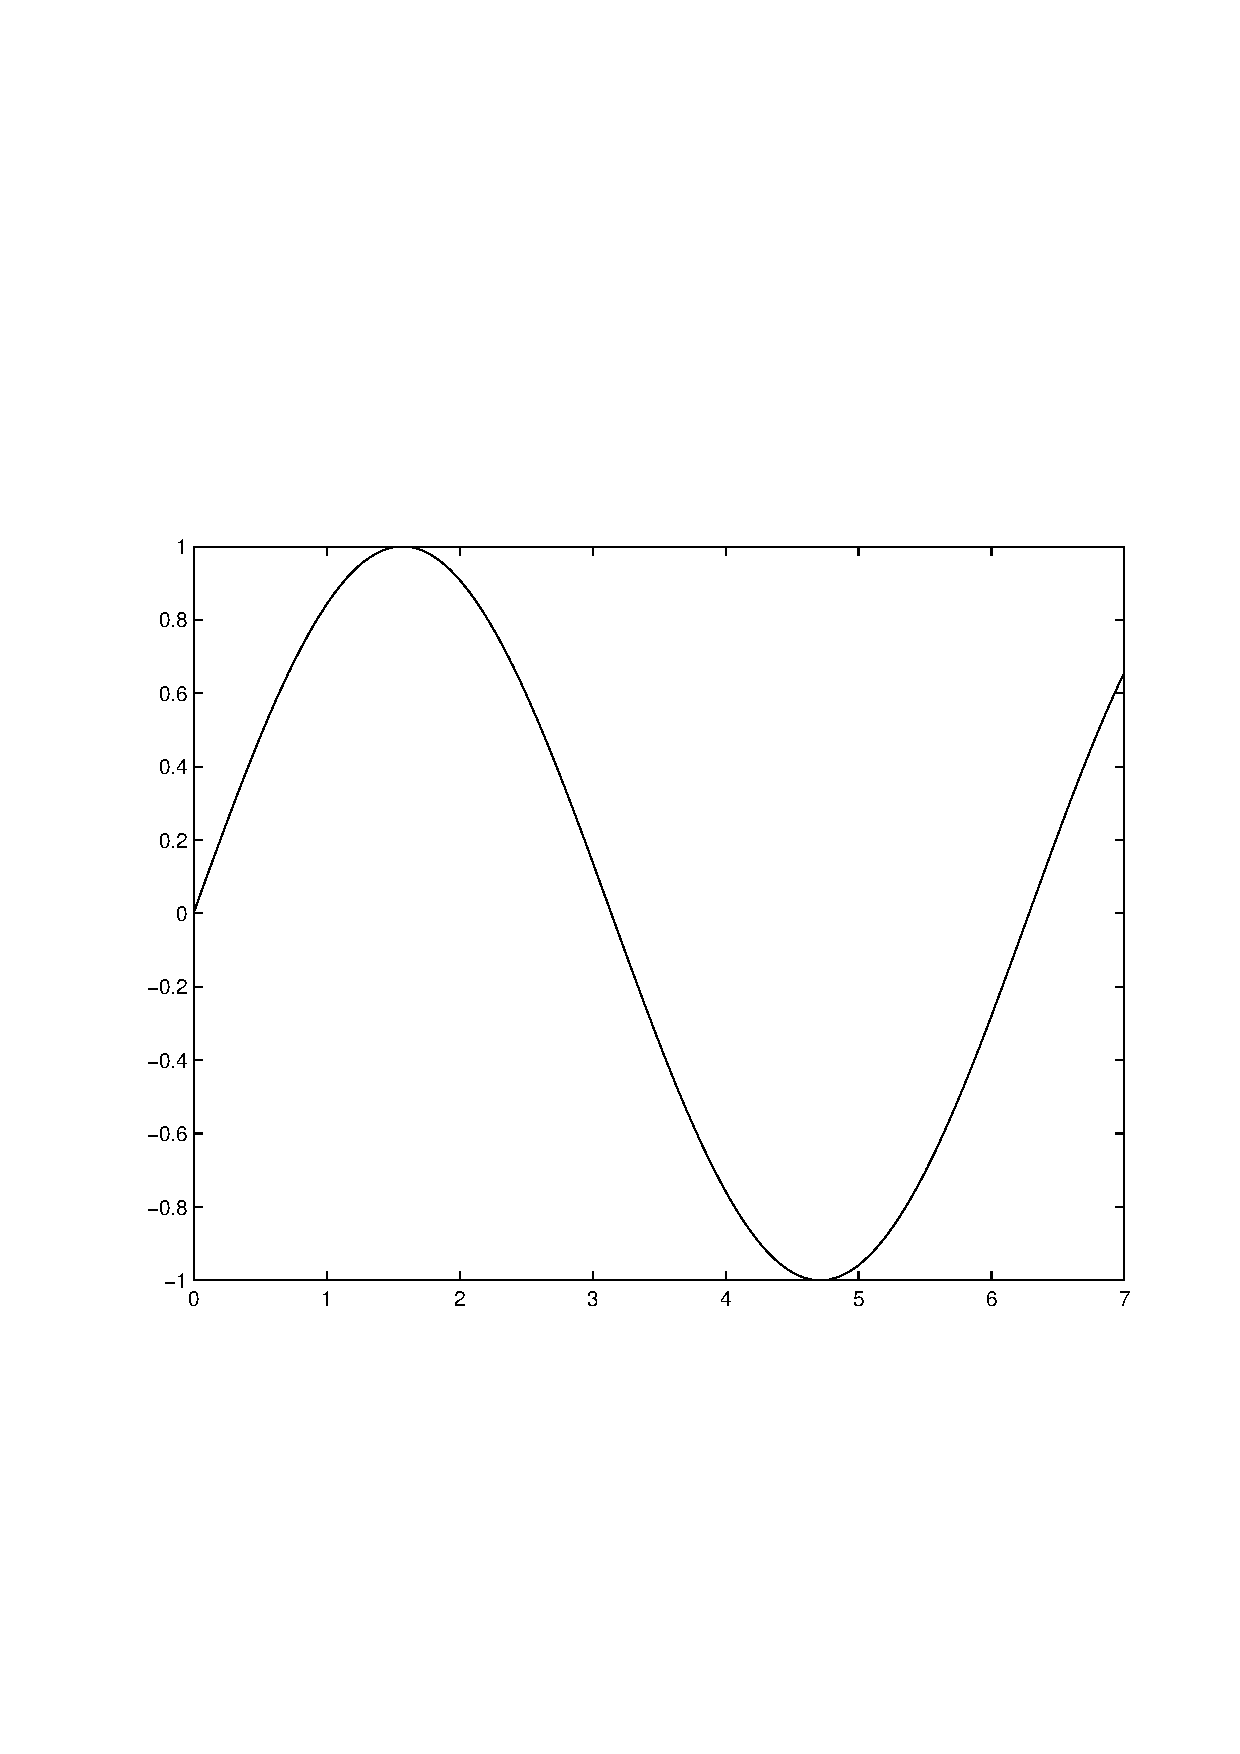
\includegraphics[width=5cm,height=3cm]{figs/fig}
\caption{Sub-figure 2\label{fig:float2-2}}
\end{minipage}
\end{figure}

\begin{figure}
  \subfigure[Small Box with a Long Caption]{
    \label{fig:mini:subfig:a} %% label for first subfigure
    \begin{minipage}[b]{0.4\textwidth}
      \centering
      \includegraphics[width=1in]{figs/sin}
    \end{minipage}}%
  \subfigure[Big Box]{
    \label{fig:mini:subfig:b} %% label for second subfigure
    \begin{minipage}[b]{0.4\textwidth}
      \centering
      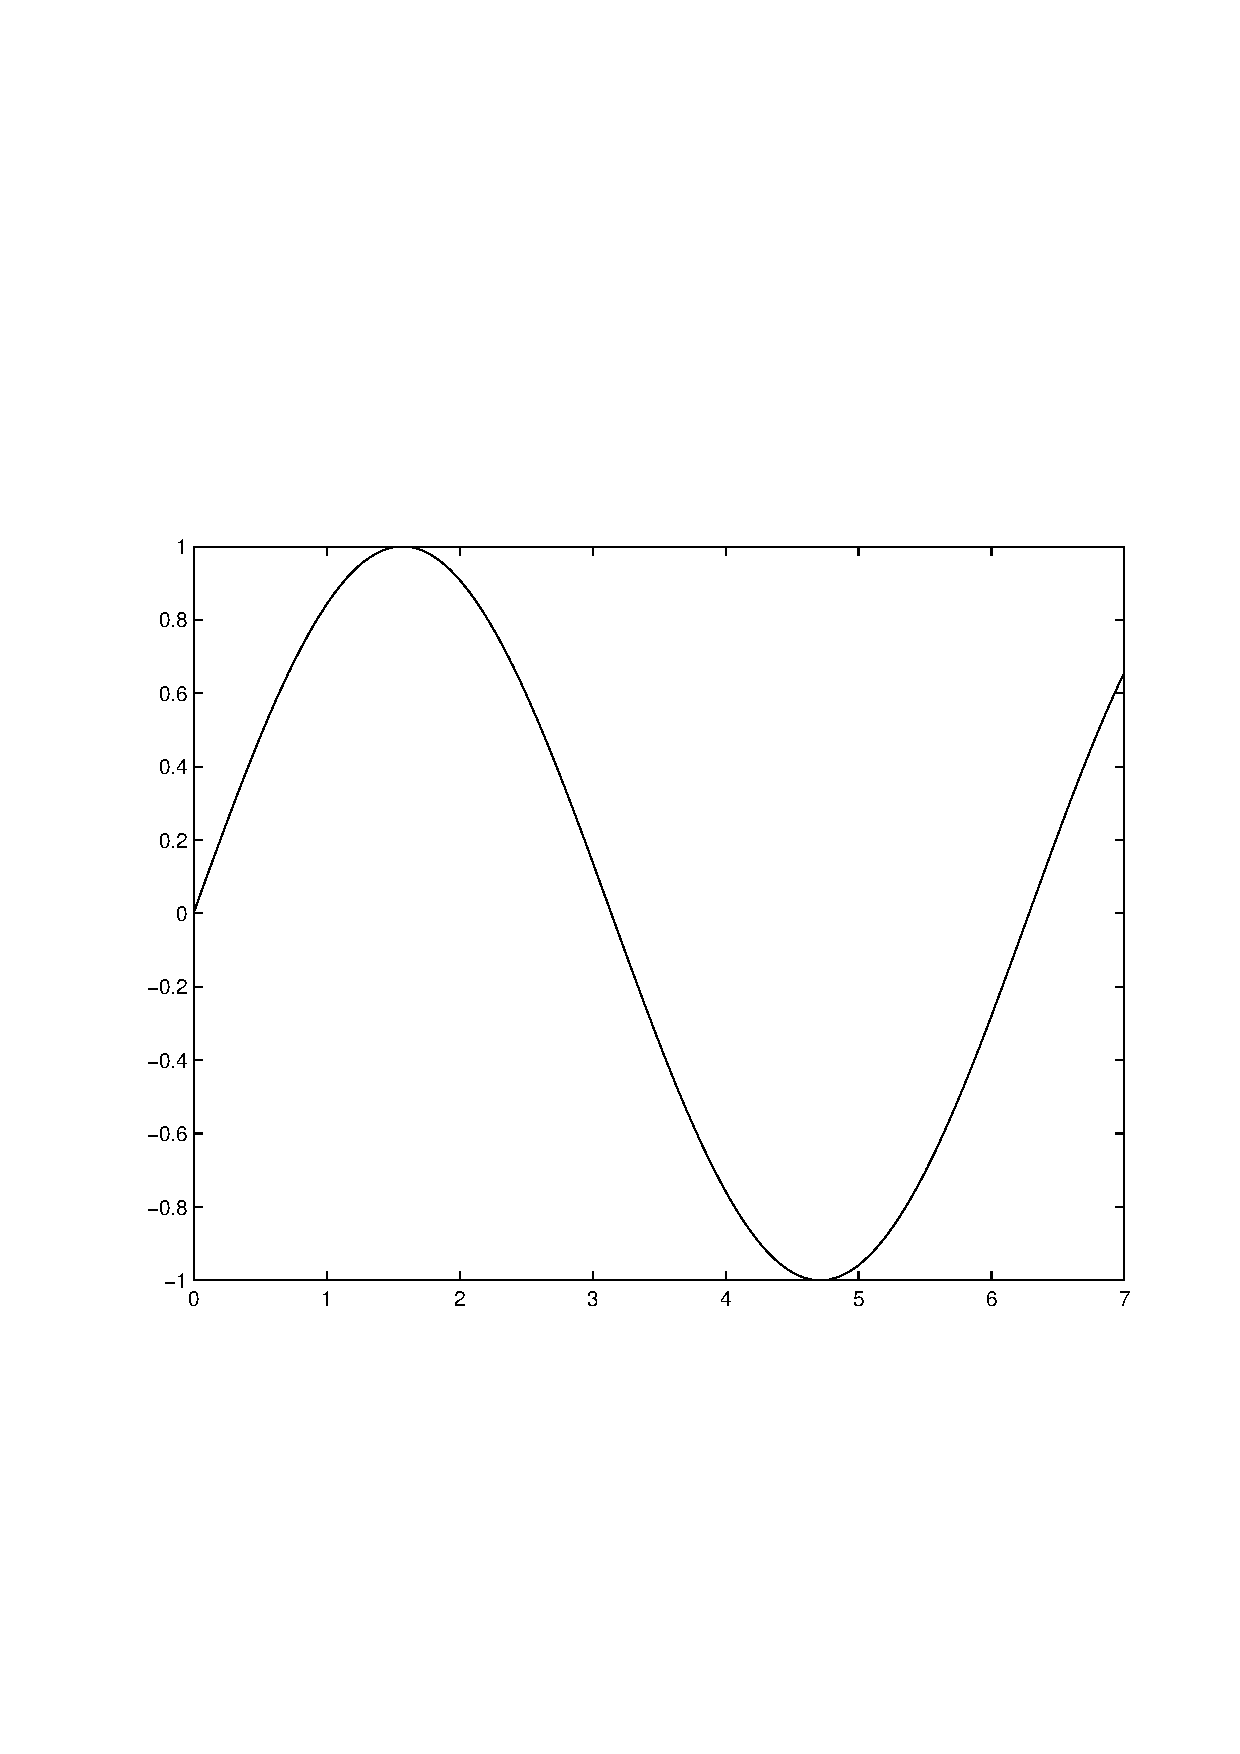
\includegraphics[width=1in]{figs/fig}
    \end{minipage}}
  \caption{Minipages Inside Subfigures}
  \label{fig:mini:subfig} %% label for entire figure
\end{figure}

\acknowledgements{\authorthanks} % 

\BeginRef
\bibitem{[1]} Aizicovici, S. and  Staicu,  V.,  Multivalued evolution equations with nonlocal initial conditions in Banach spaces,
{\it NoDEA Nonlinear Differential Equations Appl.}, 2007, 14(3): 361-376.

\bibitem{[2]} Balachandran, K., Park, J.Y. and  Trujillo, J.J.,  Controllability of nonlinear fractional dynamical systems, {\it Nonlinear Anal.}, 2012, 75(4): 1919-1926.

\bibitem{[3]} Byszewski, L. and  Lakshmikantham, V.,  Theorem about the existence and uniqueness of solutions of a nonlocal Cauchy problem in a Banach space, {\it Appl.\ Anal.}, 1990, 40(1): 11-19.

\bibitem{[4]} Chen, L.Z. and Fan, Z.B.,  On mild solutions to fractional differential equations with nonlocal conditions, {\it Electron.\ J.\ Qual.\ Theory Differ.\ Equ.}, 2011, 2011(53): 1-13.

\bibitem{[5]} Chen, L.Z., Fan, Z.B. and Li, G., On a nonlocal problem for fractional differential equations via resolvent operators,  {\it Adv.\ Difference Equ.},  2014, 2014: Article ID 251, 12 pages.

\EndRef
%%%%%%%%%%%%%%%%%%%%%%%%%%%%%%%%%%%%%%%%%%
\end{document}